\chapter{Implémentation du M1}
\section{Démarche modélisation M1}
L'énoncé du projet/TP nous propose un serveur avec les fonctionalité suivantes :

\begin{itemize}
\item
  Gestion des connexions, nous la nommerons \verb+ConnexionManager+.
\item 
 Gestion de la base de données (\verb+Database+).
\item
  Gestion d'un système de sécurité (\verb+SecurityManager+).
\end{itemize}

Un composant étant par définition une spécification d'une ou plusieurs fonctionalités, nous avons intuitivement construit notre M1 autours de ces trois instances de \verb+Composant+ listée précédement.


\section{Diagramme M1}
\pagestyle{empty}
%\newgeometry{a3paper}
\begin{figure}[htb]
%\centering
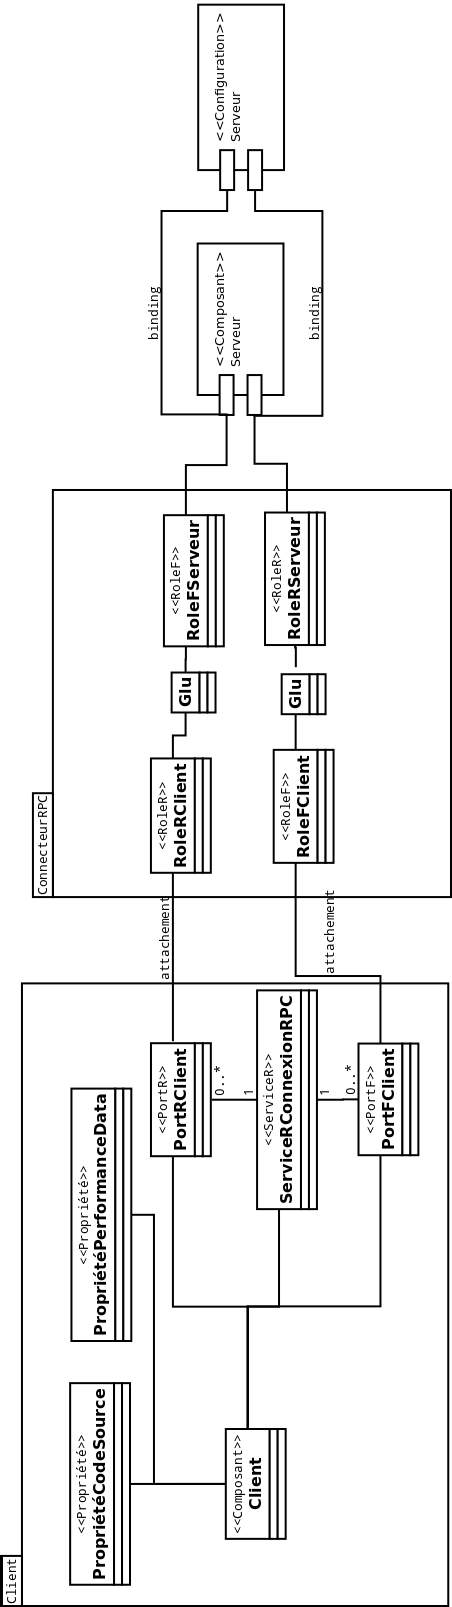
\includegraphics[scale=0.20]{img/M11}
\end{figure}
